\documentclass[]{article}
\usepackage{lmodern}
\usepackage{amssymb,amsmath}
\usepackage{ifxetex,ifluatex}
\usepackage{fixltx2e} % provides \textsubscript
\ifnum 0\ifxetex 1\fi\ifluatex 1\fi=0 % if pdftex
  \usepackage[T1]{fontenc}
  \usepackage[utf8]{inputenc}
\else % if luatex or xelatex
  \ifxetex
    \usepackage{mathspec}
  \else
    \usepackage{fontspec}
  \fi
  \defaultfontfeatures{Ligatures=TeX,Scale=MatchLowercase}
\fi
% use upquote if available, for straight quotes in verbatim environments
\IfFileExists{upquote.sty}{\usepackage{upquote}}{}
% use microtype if available
\IfFileExists{microtype.sty}{%
\usepackage{microtype}
\UseMicrotypeSet[protrusion]{basicmath} % disable protrusion for tt fonts
}{}
\usepackage[margin=1in]{geometry}
\usepackage{hyperref}
\hypersetup{unicode=true,
            pdftitle={MT7027: Project 1},
            pdfauthor={Anton Stråhle, Jan Alexandersson \& Max Sjödin},
            pdfborder={0 0 0},
            breaklinks=true}
\urlstyle{same}  % don't use monospace font for urls
\usepackage{longtable,booktabs}
\usepackage{graphicx,grffile}
\makeatletter
\def\maxwidth{\ifdim\Gin@nat@width>\linewidth\linewidth\else\Gin@nat@width\fi}
\def\maxheight{\ifdim\Gin@nat@height>\textheight\textheight\else\Gin@nat@height\fi}
\makeatother
% Scale images if necessary, so that they will not overflow the page
% margins by default, and it is still possible to overwrite the defaults
% using explicit options in \includegraphics[width, height, ...]{}
\setkeys{Gin}{width=\maxwidth,height=\maxheight,keepaspectratio}
\IfFileExists{parskip.sty}{%
\usepackage{parskip}
}{% else
\setlength{\parindent}{0pt}
\setlength{\parskip}{6pt plus 2pt minus 1pt}
}
\setlength{\emergencystretch}{3em}  % prevent overfull lines
\providecommand{\tightlist}{%
  \setlength{\itemsep}{0pt}\setlength{\parskip}{0pt}}
\setcounter{secnumdepth}{0}
% Redefines (sub)paragraphs to behave more like sections
\ifx\paragraph\undefined\else
\let\oldparagraph\paragraph
\renewcommand{\paragraph}[1]{\oldparagraph{#1}\mbox{}}
\fi
\ifx\subparagraph\undefined\else
\let\oldsubparagraph\subparagraph
\renewcommand{\subparagraph}[1]{\oldsubparagraph{#1}\mbox{}}
\fi

%%% Use protect on footnotes to avoid problems with footnotes in titles
\let\rmarkdownfootnote\footnote%
\def\footnote{\protect\rmarkdownfootnote}

%%% Change title format to be more compact
\usepackage{titling}

% Create subtitle command for use in maketitle
\newcommand{\subtitle}[1]{
  \posttitle{
    \begin{center}\large#1\end{center}
    }
}

\setlength{\droptitle}{-2em}

  \title{MT7027: Project 1}
    \pretitle{\vspace{\droptitle}\centering\huge}
  \posttitle{\par}
    \author{Anton Stråhle, Jan Alexandersson \& Max Sjödin}
    \preauthor{\centering\large\emph}
  \postauthor{\par}
    \date{}
    \predate{}\postdate{}
  

\begin{document}
\maketitle

\section{Introduction}\label{introduction}

In this project we are dealing with data concerning two different
insurance branches collected over 10 years. We do not know anything
about the sizes of the two insurance portfolios except the fact that
their size has not changed over the decade which the data spans.
Furthermore, the insurance products are of the non-life type and are
paid out in lump payments.

\section{Exercise 1}\label{exercise-1}

In this exercsie we want to find trends in the data for the two
insurance branches in order to model future claims in a block-wise
manner. Since the data is structured in a way such that we only have the
claim day (i.e. \(1,2,...,3650\)) we assume that 365 day/year and that a
month is 365/12 days (to get 12 months).

\includegraphics{Projekt1_files/figure-latex/unnamed-chunk-2-1.pdf} From
the previous histograms it seems reasonable to divide the months into
two homogenous groups with their own claim processes. One group for
months \((1-4, 9-12)\) and one for months \((5-8)\). We also wish to
examine if we have homogeneity between the different years during which
the claim data was collected.

\includegraphics{Projekt1_files/figure-latex/unnamed-chunk-3-1.pdf}
\includegraphics{Projekt1_files/figure-latex/unnamed-chunk-3-2.pdf}

\begin{verbatim}
## $y
## [1] "Counts"
## 
## attr(,"class")
## [1] "labels"
\end{verbatim}

We note from the previous plots that there does not seem to be any major
difference in the number of claims between the years.

We now wish to fit homogeneous Poisson distributions \(N_ij\) (where
\(i\) represents the insurance type and \(j\) represents the season) to
the months of each season and each insurance product.

\[
N_{ij} \sim \text{Po}(\lambda_{ij})
\]

\includegraphics{Projekt1_files/figure-latex/unnamed-chunk-4-1.pdf}
\includegraphics{Projekt1_files/figure-latex/unnamed-chunk-4-2.pdf}
\includegraphics{Projekt1_files/figure-latex/unnamed-chunk-4-3.pdf}
\includegraphics{Projekt1_files/figure-latex/unnamed-chunk-4-4.pdf}

The Poisson variables which have been fit for the different seasons and
insurance branches have had their parameter \(\lambda_{ij}\) estimated
through maximum-likelihood methods using the data from the 10 previous
years. We note that we seem to have overdispersion for \(N_{11}\) and
\(N_{12}\), meaning that the variance is not truly equal to the
expectation which is the case for a Poisson variable. For \(N_{21}\) and
\(N_{22}\) date does however seem to indicate that we have
underdispersion, meaning that the variance is lower than the
expectation.

To solve this we fit negative binomial distributions to \(N_{ij}\) as
this distribution does not have the property of equal expectation and
variance as the Poisson distribution does.
\includegraphics{Projekt1_files/figure-latex/unnamed-chunk-5-1.pdf}
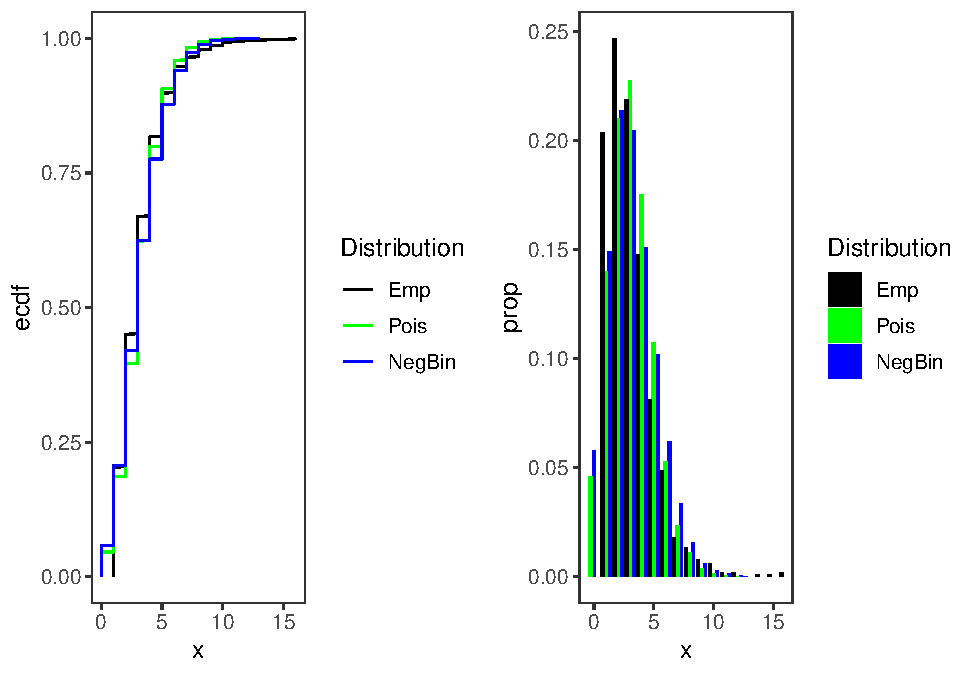
\includegraphics{Projekt1_files/figure-latex/unnamed-chunk-5-2.pdf}
\includegraphics{Projekt1_files/figure-latex/unnamed-chunk-5-3.pdf}
\includegraphics{Projekt1_files/figure-latex/unnamed-chunk-5-4.pdf}

\section{Exercise 2}\label{exercise-2}

It is not only of interset to observe the number of claims over time but
to also examine the sizes of these claims.

\includegraphics{Projekt1_files/figure-latex/unnamed-chunk-6-1.pdf}
\includegraphics{Projekt1_files/figure-latex/unnamed-chunk-6-2.pdf}

It seems as if the avergae claim costs are time independent, atleast
when aggregated on a monthly basis, from the two previous plots. We can
also observe the mean of the claim sizes for every day in order to
further strengthen the assumption of time independence.

\includegraphics{Projekt1_files/figure-latex/unnamed-chunk-7-1.pdf}
\includegraphics{Projekt1_files/figure-latex/unnamed-chunk-7-2.pdf}

We note from the figures that the average claim sizes seem to be time
independet. An interesting factor is however that all extremely
deviating claim costs seem to occur during the summer (i.e period 2). In
conclussion it seems as if the claim costs are independent of time.
Another thing that we want to examine is whether or not we have
independence between the average claim costs and the number of claims.

\includegraphics{Projekt1_files/figure-latex/unnamed-chunk-8-1.pdf}

We note that we do not seem to have any systematic correlation for any
of the combinations of claims and claim costs, meaning that we can model
the number of claims and the claim costs independently.

\section{Exercise 3}\label{exercise-3}

\includegraphics{Projekt1_files/figure-latex/unnamed-chunk-9-1.pdf}

We note from the figures above that there seems to be some kind of
positive correlation between the two insurance products, meaning that we
cannot model the claims for each product separatley, but that we instead
have to model the jointly. We can however still model the claim costs of
the two branches independently as we saw in the previous exercise.

\section{Exercise 4}\label{exercise-4}

As we mentioned previously the number of claims for the two branches are
not independent, meaning that the have to be sampled from a bivariate
distribution rather than two univariate distributions. This can be done
by either deriving the bivariate distribution analytically and then
sampling from it or, as we will do, by using a bootstrap sampler. We
begin by sampling the number of claims for each month of the following
year from the data of the correct season.

\includegraphics{Projekt1_files/figure-latex/unnamed-chunk-10-1.pdf}

\section{Exercise 5}\label{exercise-5}

We now want to implement two separate XL-covers. The first cover caps
losses for the \(10\%\) worst claims. For our two branches these cut-off
\(M_1\) and \(M_2\) are the following

\begin{longtable}[]{@{}rr@{}}
\caption{Cut-offs}\tabularnewline
\toprule
Type & M\tabularnewline
\midrule
\endfirsthead
\toprule
Type & M\tabularnewline
\midrule
\endhead
1 & 44512\tabularnewline
2 & 153871\tabularnewline
\bottomrule
\end{longtable}

\includegraphics{Projekt1_files/figure-latex/unnamed-chunk-12-1.pdf}

From the figure above we see the distribution of claim costs for the two
branches with, and wihtout, XL-cover. Of course these covers come at a
price which we can estimate from histrocial data.

\begin{longtable}[]{@{}rr@{}}
\caption{Prices for the two XL-covers}\tabularnewline
\toprule
Type & Price\tabularnewline
\midrule
\endfirsthead
\toprule
Type & Price\tabularnewline
\midrule
\endhead
1 & 9443163\tabularnewline
2 & 53101874\tabularnewline
\bottomrule
\end{longtable}

We then want to examine how the purchase of these XL-covers would impact
our total losses for the forthcoming year. We saw a simulated
distirbution of the losses without the XL-covers in figure 1. If we
implement the covers we get the following simulated distributions.

\includegraphics{Projekt1_files/figure-latex/unnamed-chunk-14-1.pdf}
\includegraphics{Projekt1_files/figure-latex/unnamed-chunk-14-2.pdf}
\includegraphics{Projekt1_files/figure-latex/unnamed-chunk-14-3.pdf}

We see that the distribution is lighter-tailed which of course is to be
expected after the purchase of an XL-cover.

\section{Exercise 6}\label{exercise-6}

We now want to implement an SL-cover instead of an XL-cover for both
insurance branches. Like the XL-covers the SL-covers insure against the
\(10\%\) worst annual costs at a price of \(120\%\) of the expected
cost.

The prices of these two SL-covers do of course come at a cost.

\begin{longtable}[]{@{}rr@{}}
\caption{Prices for the two SL-covers}\tabularnewline
\toprule
Type & Price\tabularnewline
\midrule
\endfirsthead
\toprule
Type & Price\tabularnewline
\midrule
\endhead
1 & 158699.9\tabularnewline
2 & 868680.8\tabularnewline
\bottomrule
\end{longtable}

\includegraphics{Projekt1_files/figure-latex/unnamed-chunk-16-1.pdf}
\includegraphics{Projekt1_files/figure-latex/unnamed-chunk-16-2.pdf}
\includegraphics{Projekt1_files/figure-latex/unnamed-chunk-16-3.pdf}
\includegraphics{Projekt1_files/figure-latex/unnamed-chunk-16-4.pdf}

\section{Exercise 7}\label{exercise-7}

Lastly we want to implement an SL-cover which insured against \(10\%\)
of the worst total annual costs, i.e.~summed over both branches. This
cover will be priced and insure like the individual SL-covers in
Exercise 6.

The cost of this cover, based on historical data, is
8.8721907\times 10\^{}\{5\}

\includegraphics{Projekt1_files/figure-latex/unnamed-chunk-18-1.pdf}
\includegraphics{Projekt1_files/figure-latex/unnamed-chunk-18-2.pdf}

We see from the two histograms that the total SL-cover implies a higher
expected cost but also limits the total annual cost to \(M =\)
2.7495343\times 10\^{}\{8\}. As such a more risk averse insurance
provider might opt for the SL-cover to completly exclude the possiblity
of large deviations in the annual costs whilst a more risk-taking
insurance provide might avoid the SL-cover to reduce the expected annual
cost.


\end{document}
